\RequirePackage[2020-02-02]{latexrelease}
%\documentclass[9pt,twocolumn,twoside]{cidlab-draft}\templatetype{cidlab-invited}
\documentclass[man]{apa}

\newcommand{\hdr}{HDRP}

\title{On the transformation incoherence of the HDI+ROPE testing procedure}

\abstract{The Bayesian HDI+ROPE decision rule is an increasingly common approach to testing null parameter values. 
The decision procedure involves a comparison between a posterior highest density interval (HDI) and a pre-specified region of practical equivalence (ROPE). One then accepts or rejects the null parameter value depending on the overlap (or lack thereof) between these intervals. 
Here we demonstrate, both theoretically and through examples, that this procedure is logically incoherent.
Because the HDI is not transformation invariant, the ultimate inferential decision depends on statistically arbitrary and scientifically irrelevant properties of the statistical model.
The incoherence arises from a common confusion between probability density and probability proper.  The HDI+ROPE procedure relies on characterizing posterior densities as opposed to being based directly on probability. 
We conclude with recommendations for alternative Bayesian testing procedures that do not exhibit this pathology and provide a ``quick fix'' in the form of quantile intervals.}

\shorttitle{Transformation incoherence}

\author{Alexander Etz$^{abc}$,
Adriana F.\ Ch\'avez De la Pe\~na$^{bc}$,
Luis Baroja$^{bc}$,
Kathleen Medriano$^{bc}$,
and
Joachim Vandekerckhove$^{bc}$}

\affiliation{%
$^{a}$ Department of Psychology UT Austin\\
$^{b}$ Department of Cognitive Sciences, UC Irvine\\
$^{c}$ Department of Statistics, UC Irvine}

\leftheader{Etz}


\usepackage{
    amsmath,amssymb,amsfonts,
    centernot,csquotes,
    epsfig,epstopdf,epigraph,
    graphicx,
    longtable,
    mathtools,
    subfig,
    tikz,
    url}
\usepackage[super]{nth}
\usepackage[english]{babel}

%\epstopdfDeclareGraphicsRule{.tif}{png}{.png}{convert #1 \OutputFile}
%\AppendGraphicsExtensions{.tif}

%\newcommand{\fig}[1]{\textbf{Figure~#1}}
%\newcommand{\tbl}[1]{\textbf{Table~#1}}

\newcommand\blfootnote[1]{%
  \begingroup
  \renewcommand\thefootnote{}\footnote{#1}%
  \addtocounter{footnote}{-1}%
%  \endgroup
}



\newcommand{\citealp}[1]{\citeNP{#1}}
\newcommand{\citet}[1]{\citeA{#1}}
\newcommand{\citeyearpar}[1]{\citeyear{#1}}

\makeatletter
\def\citep{%
   \@ifnextchar[%
     {\citep@i}
     {\citep@i[]}%
}
\def\citep@i[#1]{%
   \@ifnextchar[%
     {\citep@ii{#1}}
     {\citep@ii{#1}[]}%
}
\def\citep@ii#1[#2]#3{%
  \cite<#1>[#2]{#3}%
}
\makeatother

\newcommand{\M}{\mathcal{M}}
\DeclareMathOperator*{\argmin}{arg\,min}
\DeclareMathOperator*{\argmax}{arg\,max}
\newcommand{\oddss}{\text{odds}}
\newcommand{\logit}{\text{logit}}

%\definecolor{orange2}{HTML}{F5793A}
%\definecolor{blue2}{HTML}{A95AA1}
\newcommand{\ora}[1]{{#1}}
\newcommand{\blu}[1]{{#1}}

%\newcommand{\jv}[1]{\todo[inline,color=lime]{#1 -\textit{jv}}}
%\newcommand{\afcp}[1]{\todo[inline,color=red]{#1 -\textit{adri}}}
%\newcommand{\ae}[1]{\todo[inline,color=blue]{#1 -\textit{etz}}}
%\newcommand{\lb}[1]{\todo[inline,color=orange]{#1 -\textit{lb}}}
%\newcommand{\km}[1]{\todo[inline,color=orange]{#1 -\textit{kath}}}

%\newcommand{\mdl}[1]{\todo[linecolor=red,backgroundcolor=red!25,bordercolor=red,inline]{MDL: #1}}
%\newcommand{\mv}[1]{\todo[linecolor=blue,backgroundcolor=blue!25,bordercolor=blue,inline]{MV: #1}}
%\newcommand{\afcp}[1]{\todo[linecolor=green,backgroundcolor=green!25,bordercolor=green,inline]{AFCP: #1}}
%\newcommand{\jv}[1]{\todo[linecolor=orange,backgroundcolor=orange!25,bordercolor=orange,inline]{JV: #1}}
%\newcommand{\pkm}[1]{\todo[linecolor=yellow,backgroundcolor=orange!25,bordercolor=yellow,inline]{PKM: #1 }}

\def\driftangle{\theta}
\def\nondecisiontime{\tau}
\def\driftlength{\delta}
\def\boundary{\eta}
\def\mux{\mu_x}
\def\muy{\mu_y}
\def\polar{\text{CDDM}_\circ}
\def\cartn{\text{CDDM}_+}

\graphicspath{{./p/}}

\begin{document}

%\thispagestyle{firststyle}

\maketitle

%Imagine you live in an apartment with a square living room, and you want to renovate the flooring. Such renovations would naturally require you to know the size of the room in square feet (or meters). You measure the length of one wall and find it is 20 feet long. 


%Sometimes people would like to test hypotheses
%Many research questions come down to a test of a hypothesis. 
%Do two groups have the same performance, or not? Are two measures associated, or not? These and other canonical research questions can be answered statistically using a hypothesis test. The core idea 
%This is often regarded as a good idea but not always (eg. Greenland)

\noindent The crisis of confidence in psychological science has reinflamed historical controversies surrounding the enterprise of statistical hypothesis testing.  Classical null hypothesis significance testing (NHST) has been the target of the majority of these criticisms, including that it is overly dichotomous \cite{gibson2021}, easily ``hackable'' \cite{SimmonsEtAl2011}, it can only reject and not accept the null hypothesis \cite{Rouder2009ttest}, that null hypothesis are false \textit{a priori} \cite{Cohen1994,mcshane2019}, and that it answers the wrong question because estimation is more useful \cite{Cumming2014}. %We concede these criticisms have some validity in certain cases, especially when aimed at $p$-values, but we believe that hypothesis testing still has a place in science. The important thing going forward is to use hypothesis testing procedures that have good properties at the right time.

%But not all methods for conducting hypothesis tests are created equal. There exist many ways of testing hypotheses, many of which do not rely on $p$-values. 
 %One prominent alternative is testing using Bayes factors \cite{Jeffreys1935}. Bayes factors have certain benefits including ... <Bayesian thinking being more natural.> <Coherence>%, but these have only recently seen a surge in popularity in psychology. %and \hdr{} and also others that were popular some time ago %(before the De Finetti - Lindley limit of 2020) 
%Alternative methods have been proposed to ditch p-values and improve how we conduct hypothesis tests. 

%However, Bayes factors are not without their critics. <List of some criticism.>

One prominent example is the so-called HDI+ROPE procedure (henceforth, \hdr{}) introduced by \citeA{Kruschke2011,Kruschke2013} as a superseding alternative to classical NHST.  
While we are strong proponents of the Bayesian statistical paradigm \cite{EtzSI,Vandekerckhove2018} in which \hdr{} is based, we will argue here that \hdr{} is flawed and should be avoided, on grounds similar to the above objections to NHST.  Specifically, \hdr{} can lead to inconsistent inferences that depend critically on highly arbitrary choices that must be made by the analyst about how to represent the model. 
%To give an analogy, it would be like if a casino were to estimate that the probability Germany wins the world cup is 1/6 but then not go on to give them odds to win of 1:5. 

In what follows we will first informally describe the \hdr{} with a fictional scenario that highlights its problematic nature. The example will demonstrate that multiple researchers using the \hdr{} can come to different conclusions despite employing mathematically equivalent models, priors, ROPEs, and data. %The example involves estimation of a binomial rate, similar to the initial motivating example given for the \hdr{} \cite{Kruschke2011}. %We will follow this fictional scenario with real-world examples of this problematic behavior. 

To give insight into why the inconsistent inferences using the \hdr{} occur, we will discuss the formal decision-theoretical properties of the method. The crucial flaw we highlight is that different, mathematically equivalent, representations of a hypothesis test do not lead to equivalent inferences. We show that this pathology is due to the test's reliance on probability density to determine which parameter values are ``most plausible.'' However, unlike probability (which requires that equivalent sets must have equal probabilities), probability density values may depend on how we label the parameters of a model.  Differently put, \textit{sets of parameter values with high density in one representation of the model may have low density in another}. As a result, \hdr{} can simultaneously conclude that the null hypothesis \textit{is} and \textit{is not} to be rejected, which is logically incoherent.

Finally, we propose an easy-to-implement modification of the \hdr{} that resolves the current pathology and achieves coherence. The solution is to use a test that is based on probability rather than probability density. 
%Finally, we illustrate the effect of this change using a published data set.

% HDI's reliance on the specific form of the parameterization chosen for the model. In other words, changing how we label the parameters of the model will change the set 

%* Formally describe the \hdr{} method,
 %   * HDI as a generalization of mode 
  %  * An example (standard normal and log-normal)

%* Describe a fictional but realistic scenario that highlights the problematic nature of \hdr{}
%  * Avery, Blair, and Cassidy

%* Describe real-world examples

% Why does this keep happening to me!!??.jpg

%* Discuss the decision-theoretical properties of \hdr{}
%  * Generic intro decision theory
%  * Transformation equivariance and inequivariance
%  * Transforming probabilities versus densities
%  * Graphical illustration (normal and log-normal)

% An easy fix!

%* Propose an easy-to-implement modification of the \hdr{} approach that resolves the current pathology
%  * Based on probability, not density
%  * (Similar!) Graphical illustration
  
%* Discussion + conclusion
%    * alternatively, another simple solution uses prior and posterior probabilities of being in the rope (leading to a form of a bayes factor)


%-When we have a model for some phenomenon, it specifies the probabilities of outcomes.

%-As a convenience, we use parameterized families. This way we can say a ``normal with mean zero and variance 1'' instead of writing out the function all the time.

%-We can choose different ways to represent this paramterization

%-When we reparameterize a model we are simply re-expressing the same probability function


\section*{Introduction to the \hdr{} test}

The \hdr{} test is similar in procedure to the broader category of equivalence tests \cite{RogersEtAl1993}, which can be characterized as extensions of point-null tests into tests of equivalence regions.
However, the \hdr{} test only uses the rope as a means to test a point null and does not entail acceptance or rejection of the entire region. The \hdr{} test is therefore more similar in logic to other point null tests.

An \hdr{} test can be conducted as follows.  
First, one determines a parameterized model for the data and specifies the prior distributions for the parameters. 
Then, one specifies the null hypothesis of interest as one particular parameter value. This is some specific value of the parameter that is considered especially important, such as a correlation being zero.
One then specifies a region of ``practical equivalence'' around the null value, consisting of parameter values that can be considered only negligibly different from it for practical purposes.
Then, one collects data and obtains the posterior distribution of the parameter of interest. For this step, one needs to explicitly choose a parameterization of the model to be used for the test. 
From this posterior, one constructs a highest-density interval, which is a set of parameter values where every value in the set has higher posterior density than any outside the set. 

If the HDI and ROPE do not overlap, one rejects the null hypothesis for practical purposes. If the ROPE encompasses the entire HDI, then one accepts the null for practical purposes. If the ROPE and HDI partially overlap, one reserves judgment about the status of the null hypothesis. 






% -Essentially, instead of testing one null hypothesis one tests against a collection of nulls that make up the equivalence region.

% -The equivalence region is determined by considering both relevant theory and the context of the problem, and specifying values of the parameters that should be considered equivalent to the null value for practical purposes. 

% -Finally, a decision rule is defined to determine if we should conclude that the parameter is in the equivalence region or not.

% -Different tests use different decision rules, but in the end a the equivalence region is either supported or refuted.

% -For example, probably the most common equivalence test is the ``two one-sided tests'' procedure. In this test, once the equivalence region is determined, one performs a one-sided hypothesis test against both of the endpoints. That is, one tests whether the parameter is less than the lower end point or greater than the upper end point.  
    
\subsection*{A fictional example}
    
Avery, Blair, and Cassidy are triplets who are training their pet hamster to detect by smell whether a piece of cheese is safe to eat or not. After months of training they have decided to run a rigorous, blinded experiment. They will present the hamster with 47 pieces of cheese and observe how many it identifies correctly.

To determine if their hamster has been successfully trained to detect the safety of cheese, the triplets decide to implement an \hdr{} test as outlined above for their analysis. They specify that the success or failure of a given cheese identification is modeled as an independent Bernoulli trial with probability of success $\theta$. The three decide to to use a uniform distribution from 0 to 1 as their prior distribution for $\theta$, a default specification suggested by \citeA{Jeffreys1961}. 

Next the triplets need to determine their null hypothesis and ROPE. A natural null hypothesis in this case is that the hamster is responding by chance, or in other words that $\theta=.50$. After deliberation, the triplets determine that their hamster would also be considered ``practically guessing'' if its chance to detect cheese safety is within 3\% above or below chance. Thus, they specify a ROPE that spans from $\theta=.47$ to $\theta=.53$.

During the experiment their hamster correctly determines the safety of a piece of cheese 32 times out of 47. At this point the triplets must present their results to their family, but they disagree about how it should be done. Avery is a psychologist, who feels that the most intuitive scale for the results is the probability scale $\theta$. Avery produces the plot in the top panel of Figure~\ref{fig:ropes}, showing that the HDI for the posterior of $\theta$ spans .542 to .800 and does not overlap with the ROPE. %The highest-density interval of this posterior distribution does not intersect the ROPE, and 
Thus, Avery argues, the null hypothesis can be rejected with room to spare. Their hamster really can tell when cheese is safe to eat!


Blair and Cassidy take issue with Avery's presentation of the results. Blair is a biostatistician and has extensive experience interpreting log-odds in the context of clinical trials. Thus, to Blair, it seems obvious that the results should be presented on the scale of $\logit(\theta)=\log\left(\frac{\theta}{1-\theta}\right)$, shown in the bottom left panel of Figure~\ref{fig:ropes}. In this parameterization, the test value would be 0, with a ROPE ranging from $\logit(.47)=\log\left(\frac{.47}{1-.47}\right)\approx-.12$ to $\logit(.53)\approx.12$. The lower bound for HDI for the posterior of $\logit(\theta)$ is just barely outside the ROPE, giving Blair pause. Maybe the evidence is not so strong after all. Nevertheless, this version of the test allows one to reject the null hypothesis, if only just barely.

Cassidy is a practicing doctor, and is used to presenting the uncertainty of diagnoses to patients using odds of occurrence. Thus, to Cassidy, it seems only natural to present the results on the scale of $\oddss(\theta)=\frac{\theta}{1-\theta}$. In this parameterization, the test value would be 1, with a ROPE ranging from .887 to 1.128. The HDI for $\oddss(\theta)$ spans 1.02 to 3.61, intersecting with the ROPE.%Clearly, there remains much uncertainty about the value of $\oddss(\theta)$. 
%In fact, the highest density interval is extremely wide, managing to even encompass the entire ROPE. 
It seems clear to Cassidy that there is still more data needed--at this point, judgment may  be withheld about their hamster's abilities. %before they can conclude anything with confidence about their hamster's ability.

This example highlights the critical flaw of the \hdr{} test: whether the null hypothesis is rejected depends on how one decides to portray their results. Avery and Blair are able to reject the null hypothesis when the results are presented in terms of probability of success, but Cassidy must withhold judgment when they look at the results in terms of log-odds and odds of success, respectively. With the same model, the same prior information, and the same data, the triplets come to different conclusions. In other words, their conclusions do not \textit{cohere}. 

This is not an entirely contrived example.  The values in this section are the taken from Figure~1 in the paper that first described the \hdr{} procedure \cite{Kruschke2011}.

%This results in a posterior distribution for $\theta$ that is beta(

%After deliberation, they decide that their hamster should


\begin{figure}[!!h]
    \centering
    \includegraphics[width=.45\textwidth]{theta.tif}\\
    \includegraphics[width=.45\textwidth]{logit.tif}
    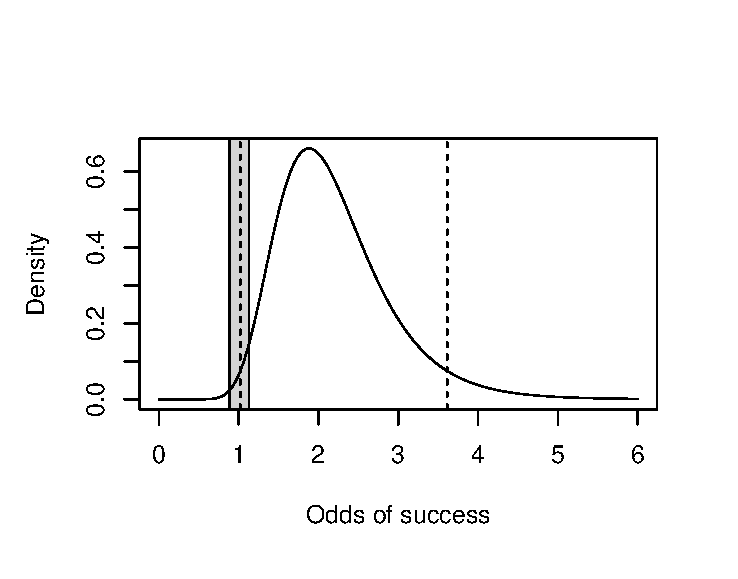
\includegraphics[width=.45\textwidth]{odds.tif}
    \caption{An illustration of the \hdr{} test. The shaded region indicates the ROPE, and the dashed line indicates the HDI of the respective posterior distributions. \textbf{Top.} $\theta$ parameterization. Test value is .50, with ROPE from .40 to .60. The 95\% HDI does not intersect the ROPE, leading to rejection of the null hypothesis. \textbf{Middle.} $\logit(\theta)$ parameterization. Test value is $\logit(.50)=0$, with ROPE from $\logit(.40)\approx-.40$ to $\logit(.60)\approx.40$. The 95\% HDI intersects the ROPE, leading to withholding judgment. \textbf{Bottom.} $\oddss(\theta)$ parameterization. Test value is $\oddss(.50)=1$, with ROPE from $\oddss(.40)=2/3$ to $\oddss(.60)=3/2$. The 95\% HDI intersects the ROPE, leading to withholding judgment.}
    \label{fig:ropes}
\end{figure}



    \subsection*{Formal description of the \hdr{} test}

We described the \hdr{} test informally above, as an assessment of how two intervals overlap. In order to describe the \hdr{} test's problem of incoherence in a precise way we will use the language of statistical decision theory. %The
%benefit of using a more formal language is that we ... 
We will begin this section with a brief introduction to decision theoretic ideas and then discuss how these ideas apply to the \hdr{} test.
 
In the language of statistical decision theory, a hypothesis testing procedure is a type of decision rule wherein the decision is a choice between one of the candidate hypotheses. If we use $\delta_T$ to represent the \textit{decision} made for test $T$, then the value of $\delta_T$ corresponds to the hypothesis chosen. For example, in the classic Neyman-Pearson testing framework one sets up a test to choose between the null hypothesis $H_0$ and the alternative hypothesis $H_1$. A test statistic ($X$), acceptance region ($R_0$) and rejection region ($R_1$) are defined. If the test statistic falls in the predefined rejection region, then $\delta_{NP}=1$ and we choose $H_1$; if the test statistic falls in the acceptance region, then $\delta_{NP}=0$ and correspondingly we choose $H_0$.% Formally, we define the decision rule as follows:

% \begin{equation*}
%     \delta_{NP} =
%     \begin{cases}
% 1 & X\in R_1\\
% 0 & X\in R_0
%     \end{cases}
% \end{equation*}


The \hdr{} test is fundamentally a hypothesis testing decision procedure and thus it can also be represented as a decision process. With the \hdr{} test we have the same hypotheses as usual. $H_0$ states that the the parameter is equal to a postulated null value $\theta_0$; $H_1$ states that the parameter takes some value other than $\theta_0$. To test these hypotheses using \hdr{} we further define a region around the null consisting of values of the parameter we consider equivalent to the null for practical purposes; this set is called a ``region of practical equivalence,'' or ROPE. We then carry out estimation of the parameter and examine if its posterior density function shows considerable overlap with the ROPE. If the areas of high density mainly lie within the ROPE, $H_0$ is accepted. If the areas of high density are largely outside the ROPE, $H_1$ is accepted. The intuition behind this procedure is seemingly straightforward: If the most plausible parameter values are practically equivalent to the null value, then it makes sense to accept it for practical purposes. Likewise, if the most plausible parameter values are not practically equivalent to the null, then reject it.

The overlap of the ROPE and the posterior distribution is formally determined by constructing a 95\% highest density interval (HDI) for the test parameter. An HDI is a set consisting of 95\% of the posterior mass, with the specific property that every parameter value in the interval has higher posterior density than any value outside the set. Formally, an HDI consisting of $\alpha$\% of the posterior mass is defined as the set  
\begin{equation}
    HDI^\alpha = \{\theta:p(\theta|D)>k_\alpha\}\label{eq:hdi}
\end{equation}
for some $k_\alpha$ chosen to satisfy the constraint $P(HDI^\alpha)=\alpha$ \cite{druilhet2007}. For notational convenience, if the $\alpha$ being used is the standard .95 we will simply write ``$HDI$'' without the superscript. 

Formally, we define the decision rule associated with the \hdr{} as follows:
\begin{equation*}
    \delta =
    \begin{cases}
    1 & \text{HDI} \centernot\cap \text{ROPE} \\ %That is an ugly negation slash but I can't find a better looking one atm
    -1 & \text{HDI} \subset \text{ROPE}\\
    0 & \text{otherwise}.
    \end{cases}
\end{equation*}
In the \hdr{} decision rule, $\delta=1$ corresponds to rejection of $H_0:\theta=\theta_0$ and $\delta=-1$ refers to its acceptance. $\delta=0$ refers to the case there is partial overlap of the sets and one must withhold judgment about the status of the null hypothesis and (if possible) collect more data until one of the other conditions is met. 
% where we withhold judgment.
%If . 

Let us revisit the hamster example with this new language. In presenting their results, Avery showed that the HDI and ROPE did not intersect for testing $\theta=.50$, and thus made the decision $\delta=1$ and rejected the null hypothesis. Blair came to a similar conclusion for testing $\logit(\theta)=0$, but the evidence did not appear as conclusive. Cassidy concluded that the HDI and ROPE partially overlapped for testing $\oddss(\theta)=1$, respectively, and thus made the decision $\delta=0$ and withheld judgment. Thus, despite having the same information, the triplets come to different conclusions about logically equivalent hypotheses despite having all of the same information. In the next section, we will provide some critical background on probability theory and use it to explain why the \hdr{} test leads to such instances of incoherence.



% Parameters : You have to decide on a way to represent the model in terms of its parameters, is it theta or is it psi or whatever.


% Using this level of analysis allows us to show that the decision (or inference) made using the \hdr{} test is dependent on our specific choice of parameterization of the model. A decision rule based on $\theta$ may not cohere with one based on $\psi$, despite both models making identical probability statements.
 


\section*{Why is the \hdr{} test incoherent?}

We will now explain the cause of the incoherent behavior exhibited by the \hdr{} test. The key idea we want to get across is that the test requires the user to find a set of parameters with ``high'' posterior density, but that there is no unique set of parameter values with the highest density. Density is a property that is determined by the parameterization of the model, which is an explicit choice made by the user of the test. As we have seen in our examples above, different choices of parameterization lead to different regions of the model with high density, which in turn leads to different conclusions from our test.

To understand why this happens, first we will review the fundamental relationship between probability and probability density. Then, we will show the difference in the way probability and probability density behave when converting from one parameterization to another. Finally, we will return to the \hdr{} test and show how it is affected by these considerations.  
    
   \subsection*{Density and probability}


\begin{figure*}[t]
    \centering
    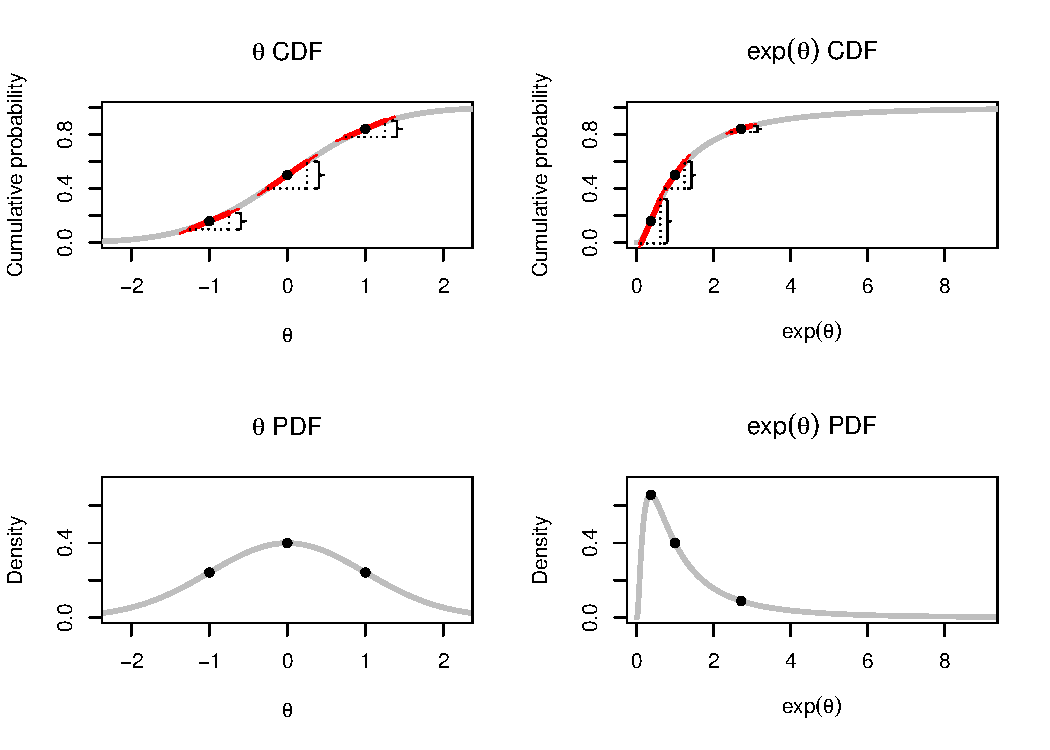
\includegraphics[width=.85\textwidth]{idunno.pdf}
    \caption{An illustration of how transformation affects the CDF and PDF. \textbf{Top left.} The CDF of a normally distributed $\theta$. \textbf{Top right.} The CDF resulting from applying the transformation $\exp(\theta)$. \textbf{Bottom left.} The PDF of a normally distributed $\theta$. \textbf{Bottom right.} The PDF resulting from applying the transformation $\exp(\theta)$.}
    \label{fig:normals}
\end{figure*}

As an illustrative example, consider that we are testing whether the mean of a normal distribution is equal to zero or not. The posterior distribution we obtain for $\theta$ from our analysis happens to be the standard normal distribution. The cumulative distribution function for a standard normal is shown in the top left panel. This function tells us for any given candidate $\theta$, the posterior probability that the ``true'' $\theta^*$ is less than $\theta$. For example, for $\theta=0$, we have $P(\theta^*<\theta|D) = .50$. This is seen in the graph by the height of the cdf curve for $\theta=0$ being at .50. We will use $F(\theta|D)$ as notation.

Recall that probability theory is fundamentally a collection of rules for assigning numbers between 0 and 1 to various sets. The cdf tells us how much probability is associated with the set of parameters whose values fall below a candidate $\theta$. Using this function, we can find the probability of other sets; the probability that $\theta$ is between any two limits $\theta_1$ and $\theta_2$ ($\theta_1<\theta_2$) can be obtained by finding how much the cdf increases as we move from $\theta_1$ to $\theta_2$; we subtract $F(\theta_1|D)$ from $F(\theta_2|D)$ to get $P(\theta_1<\theta^*<\theta_2|D)$. For instance, we take $\theta_2=.6$ and $\theta_1=.4$, then $F(.6|D)=.73$ and $F(.4|D)=.66$, giving us $P(.4<\theta^*<.6|D)=.07$. 

When the parameter space is continuous, the probability of any point is zero. However, we can look at probability density, which tells us how much probability is ``near'' a given parameter value. The idea of probability density is directly analogous to physical concepts of density, in that it tells us how much (probability) mass exists in a given region of some space. Consider our example with the standard normal posterior for $\theta$. We can take a small window $\Delta \theta$ around each $\theta$ that spans .1 below and .1 above, and find the probability that $\theta^*$ is between those limits. Some examples are drawn on the top left panel for $\Delta\theta=.2$. Regions that are more dense will have more probability.

``Near'' $\theta=-1$, there is $5\%$ of our total probability. ``Near'' $\theta=0$ there is $8\%$ of our total probability. This distribution is symmetric around 0, so ``near'' $\theta=1$, there is again $5\%$ of our total probability. If we take these amounts and divide them by the length of the window $\Delta \theta$, we have an idea of how densely the probability is packed around each of these values. We can compute the density of these windows around  $-1$, 0, and $1$ to be .25, .4, and .25, respectively. 

Thinking in terms of the cdf, how dense a region is around a parameter corresponds to how much change the function height undergoes near that point. The idea of probability density follows this line of thinking into the limit of smaller and smaller windows around $\theta$ values; we look at how much the cdf's value is changing with an infinitesimally small change around the parameter value. In other words, we look at the slope of the cdf at a given parameter value to find its density. Thus, the posterior density function is the derivative (slope, or rate of change) of the cumulative density function. In this way, an individual parameter value can have a non-zero density, and this distinguishes probability density from probability.

To recap, the density of candidate parameter values is determined by first defining a window length to be applied to the regions of $\theta$ (i.e., $\Delta\theta$), finding the probability mass within that window, and then passing on to a limit. This results in taking the derivative of the cdf. Again, this tells us how much probability is in a very small window ``near'' each candidate $\theta$ value. As we can see for our standard normal example, the highest-density point (i.e., the mode) is at $\theta=0$ and the density gradually and symmetrically decreases in either direction.

The difference in the way transformations act on probabilities and probability densities is central to our argument. Equivalent sets of parameters must naturally have equivalent probabilities, but their densities can be quite different.

    
   \subsection*{Reparameterization and transformation of variables}
Probability density quantifies how much probability mass is ``near'' a point in the support of a probability distribution. When the probability distribution is a prior or posterior distribution of a parameter, it is tempting to think of the density as a measure of how ``plausible'' each parameter value is. The problem with this line of thinking becomes clear when we realize that a parameterization of a model is merely an indexing system of a family of distributions that could have generated the data. Usually when we talk about inference, we make reference to parameter values such as $\theta$; however, what we are actually interested in is the data generating process for the data, $f(x|\theta)$. For example, in a $t$-test we may make an inference on whether the difference between group means $\mu_1$ and $\mu_2$ equals zero, but this is merely an expedient way of determining whether $f(x|\mu_1)$ is the same function as $f(x|\mu_2)$. A parameter does not exist outside of a model for some data generating process. 

When we think of parameterizations as indices of data generating processes, it becomes clear that we have to make a choice of which index to use in any given case. It may be that we choose based on convention or ease of interpretability, but we must make a choice; there is no God-given parameterization. And in making our choice, we must recognize that other analysts may make different choices. We may prefer to think of the model in terms of a $\theta$, but someone else may prefer to think in terms of $\psi$ that is some function of $\theta$. In the case that this function is bijective (both one-to-one and onto), we can say that $\psi$ is a \textit{reparameterization} of the model based on $\theta$. 

Let's consider what happens to our posterior distribution when we reparameterize the model in terms of $\exp{(\theta)}$. 
The top right panel shows the cdf of the posterior distribution for this new parameterization. Note that the only change is to scrunch and stretch the axis in different regions. 
The height of the curve has no need of adjustment. Naturally, the probability that $\theta<0$ is just the probability that $\exp{(\theta)}<1$. This makes sense, as all we have done is assigned a new labeling scheme for the model, going from $f(x|\theta)$ to $f(x|\psi)$.
For example, the data generating processes that have a $\theta$ smaller than 0 are precisely those that have a $\psi$ less than 1. 
 
In contrast to the simple way probability is maintained through transformation, the new density is not as straightforward.
Remember, density is telling us how much probability is ``near'' different parameter candidates, and what is considered ``near'' a parameter value is defined as a window of width $\Delta$.
The critical problem for thinking about plausibility in terms of density is this: data generating processes that are ``near'' one another in terms of $\theta$ may not be nearby in terms of $\psi$. 
Consider three the $\theta$ values of $-1$, 0, and 1. In this space (represented by the axis in Figure~\ref{fig:normals}), the data generating process corresponding to $\theta=-1$ and $\theta=1$ are equally far from the one corresponding to $\theta=0$.
But the data generating process corresponding to $\psi=\exp{(0)}=1$ is now much closer to the one corresponding to $\psi=\exp{(-1)} = .37$ than it is to $\psi=\exp{(1)}= 2.7$.
However, critically, the probability mass of this interval must stay the same, as equivalent sets must have equal probabilities. Thus, the probability mass in the smaller region of $\psi$ between $\exp{(-1)}$ and $\exp{(0)}$ must be more dense than the equally probable but more spread out region between $\exp{(0)}$ and $\exp{(1)}$. This is the whole idea of density: the same amount of mass in a smaller region is more dense. 

The story is the same as we shrink the window $\Delta\psi$ in the limit to find the density function. Because the probability mass has been stretched and scrunched differently in different regions of parameter space, some data generating processes that had high (low) density when expressed in terms of $\theta$ may have low (high) density when expressed in terms of $\psi$.
From the $\psi$ perspective, the densest region of parameter space is at $\exp{(-1)}$. The data generating process corresponding to $\psi=\exp{(-1)}$ has the most probability ``around'' it. 

So far we have given an intuition of the idea of how posterior density changes when we transform our parameterization or representation of the model. Essentially, we have to ensure that we account for the stretching being done to the parameter space; regions that stretch out must become less dense, and regions scrunching up must become more dense. 
In the limit, as we look at smaller neighborhoods around the parameter values, we have to make finer grained adjustments to the density. The limiting adjustment is a factor called a \textit{Jacobian} that corrects the density up or down to the extent that the neighborhood around the given parameter is shrinking or expanding (see the box ``The Jacobian and coherence'' on p.~\pageref{box:jacobian}). 

The Jacobian can have a very different effect on different regions of the new parameter space depending on the transformation. It is perhaps insightful to see the Jacobian works for a few points in the transformation of the parameter spaces for Avery and Cassidy from our hamster example earlier. In transforming from $\theta$ to $\oddss(\theta)$, calling $\gamma=\frac{\theta}{1-\theta}$, the Jacobian is $1/(1+\gamma)^2$. The point $\theta=.50$ for Avery goes to the new point $\gamma=1$ for Cassidy, and in doing so it undergoes a density adjustment factor of $1/(1+1)^2 = 1/4$. The point $\theta=.70$ for Avery goes to the point $\gamma=7/3$ for Cassidy, with a Jacobian adjustment of $1/(1+7/3)^2=.09$. Finally, the point $\theta=.90$ goes to the new point $\gamma=9$ with a Jacobian adjustment of $1/100$. %; due to the Jacobian, the highest density point for Avery has become a point with relatively low density for Cassidy (see Figure~\ref{fig:ropes}). 
The Jacobian is acting more strongly on the larger values of the parameter because the transformation of the space becomes more exaggerated as one approaches the boundary of $\theta$. Consider that $\theta=.9$ goes to $\gamma=9$, $\theta=.95$ goes to $\gamma=19$, and $\theta=.99$ goes to $\gamma=99$. The probability around these points is being stretched across larger and larger regions, so the density must be adjusted downwards accordingly. 

If we were to think of plausibility in terms of density, we would have to interpret the transformation from one parameterization to another as providing some new information. It would be as if the Jacobian is another source of data. But, critically, the adjustment due to Jacobian does not introduce any new information; its sole purpose is to ensure that the probability density function integrates to 1. 

%\begin{figure}[!!h]
%\begin{framed}
%\label{box:jacobian}
\subsection{The Jacobian and coherence.} We now give a formal definition of the Jacobian in the context of the log-normal example above. If a univariate random variable $X$ has probability density function $f_X(x)$, then the density function of the random variable $Y=g(X)$, for a smooth function $g$ with inverse $X = h(Y)$, is 
\begin{eqnarray}\label{eq:jacobian}
f_Y(y) = f_X(h(y))  \left|J(y)\right|.
\end{eqnarray}
The term $J(y) = dh(y)/dy$ is known as the \blu{\textit{Jacobian}} of the transformation, and rescales the density function to ensure that the total probability mass remains 1. The Jacobian factor is a function of the new parameter, meaning its value depends on where in the parameter space we are; neighborhoods that are shrinking will have a Jacobian greater than 1, and neighborhoods that are expanding will have a Jacobian less than 1.

Let us continue with our example of transforming from a normal random variable to a log-normal. Let $X$ follow a normal distribution with mean $\mu$ and variance $\sigma^2$, i.e., $X\sim N(\mu,\sigma^2)$. The density function of $X$ is 
\begin{eqnarray*}
f_X(x) = \frac{1}{\sqrt{2\pi\sigma^2}}\exp\left\{-\frac{1}{2\sigma^2}(x-\mu)^2\right\},
\end{eqnarray*}
for $-\infty < x < \infty$. If we were to consider where the mode of this distribution is, we would find the value of $x$ making $\exp\{-(x-\mu)^2\}$ the largest, which can be shown to be when $x=\mu$.  

Consider the change of variable $Y=e^X$, which corresponds to the fifth row of the transformations table with $a=1$. Thus, we have inverse $X=\log(Y)$ and a Jacobian equal to $1/Y$. Equation~\ref{eq:jacobian} tells us that the density function of $Y$ is given by
\begin{eqnarray*}
f_Y(y) &=&  \frac{1}{\sqrt{2\pi\sigma^2}}\exp\left\{-\frac{1}{2\sigma^2}\Big(\left(\ora{\log(y)}\right)-\mu\Big)^2\right\}\cdot\left|\blu{\frac{1}{y}}\right|\\
&=& \frac{1}{\blu{y}\sqrt{2\pi\sigma^2}}\exp\left\{-\frac{1}{2\sigma^2}\Big(\ora{\log(y)}-\mu\Big)^2\right\},
\end{eqnarray*}
for $0<y<\infty$. It can be shown that the mode of this new density is at $y=\exp{(\mu-\sigma^2)}$. 

If we were to interpret density as an indication of ``plausibility,'' then the point with highest density should be considered the ``most plausible'' value of a random variable (i.e., the mode). We would then have to simultaneously believe that the most plausible value of $X$ is $\mu$, but that the most plausible value of $Y=\exp{(X)}$ is not $\exp{(\mu)}$, but the potentially very different $\exp{(\mu-\sigma^2)}$. These two beliefs are contradictory, so treating density as a measure of plausibility is not a coherent system of reasoning.

%\end{framed}
%\end{figure}

\begin{table}[bth]
\centering 
\begin{tabular}{llll}
Transformation & Inverse function & Jacobian & Type of transformation  \\ 
\hline
$Y = g(X)$ & $X = h(Y)$ & $J(Y) =\frac{dh(Y)}{dY}$ &  \\
$Y=aX +b$  & $X= \frac{Y-b}{a}$ & $J(Y)=\frac{1}{a}$ & Linear \\
$Y= X^a$   & $X = Y^{1/a}$      & $J(Y)=\frac{1}{a} Y^{\frac{1-a}{a}}$ & Nonlinear \\
$Y= X^{1/a}$ & $X = Y^{a}$ & $J(Y)=a Y^{a-1}$ & Nonlinear \\
$Y = e^{aX}$ & $X = \frac{1}{a}\log(Y)$ & $J(Y)=\frac{1}{aY}$& Nonlinear \\
$Y = a\log(X)$  & $X = e^{Y/a}$ & $J(Y)=\frac{1}{a}e^{Y/a}$& Nonlinear \\
$Y = \frac{X}{1-X}$ & $X = \frac{Y}{1+Y}$  & $J(Y)=\frac{1}{(1+Y)^2}$ & Nonlinear\\
$Y = \frac{X}{1+X}$ & $X = \frac{Y}{1-Y}$ & $J(Y)=\frac{1}{(1-Y)^2}$& Nonlinear\\
$Y = \log\left(\frac{X}{1-X}\right)$ & $X = \frac{1}{1+e^{-Y}}$ & $J(Y)=\frac{e^{-Y}}{\left(1+e^{-Y}\right)^2}$& Nonlinear \\
$Y = \frac{1}{1+e^{-X}}$ & $X = \log\left(\frac{Y}{1-Y}\right)$ & $J(Y)=\frac{1}{Y(1-Y)}$& Nonlinear\\
%$Y = a\Phi^{-1}(X)+b$ & $X = \Phi(\frac{Y-b}{a})$ & $J(Y)=\frac{1}{a}\phi\left(\frac{Y-b}{a}\right)$\\
$Y = \Phi^{-1}(aX+b)$ & $X = \frac{\Phi(Y)-b}{a}$  & $J(Y)=\frac{1}{a}\phi(Y)$& Nonlinear\\
\end{tabular}
\caption{Common transformations and their corresponding Jacobian factors. The first column lists various transformations in the form $Y=g(X)$. The second column lists the inverse functions, $X=h(Y)$. The third column lists the Jacobian factors corresponding to each transformation, obtained by taking the derivative of the corresponding inverse function (see the explanation in the main text). Note that $\Phi$ is the normal CDF and $\phi$ is the normal PDF.}
\label{tab:transformations}
\end{table}


 % We distinguish here between the models/param
 %we need to connect the models to the sets of parameters and show why they have to keep the same probability


 \subsection*{Issues with the density-based \hdr{} test}
       % The highest-density interval contains all of those $\theta$ values for which the posterior 

As we have shown in the discussions above on density and transformation, regions of parameter space with ``high'' or ``low'' density depends on how you choose to parameterize the data generating process. The rank ordering of density can change drastically across reparameterizations of the model, meaning any inferences based directly on density are essentially artifacts of a statistically arbitrary parameterization choice. 

The \hdr{} test relies on the determination of overlap between a high-density region and an ``equivalency'' region of the parameter space. The issue with the test is now apparent: regions of parameter space can have high density in one parameterization and low density in another, meaning the location of the HDI relative to the ROPE is dependent on an arbitrary parameterization choice.  Thus, the inference one draws from the \hdr{} test is not invariant to reparameterization of the model. 

In fact, the non-invariance of the \hdr{} test to reparameterization suggests that the way we have written the decision rule associated with the test in the earlier section is incomplete; the entire decision process should be indexed by the parameterization choice made. Thus, the HDI should be explicitly $\text{HDI}_\theta$, the ROPE should explicitly be $\text{ROPE}_\theta$, and the decision rule should be explicitly $\delta_\theta$. Thus, in terms of decision theory, the problem with the \hdr{} test is that with the same data and prior, it is not the case that the decision $\delta_\theta$ will necessarily be equal to the decision $\delta_\psi$ associated with a reparameterization of the model. Different analysts with the same information can come to different conclusions based entirely on their choice of parameterization.



%-Probability vs density section show how %``\textit{The} posterior density'' does not exist, merely ``\textit{a} posterior density''.



% -
% -Meaning, the outcome of the test depends on this statistically arbitrary choice. 

% %-Consider the definition of the HDI given in \ref{eq:hdi}, which finds a set of parameter values that have density larger than some benchmark $k$. 

% -For example, we could reject the hypothesis that $\theta=0$ but not $\exp(\theta)=1$, despite these being logically equivalent statements. This is incoherent.

% -There is no god-given parameterization of a model; we always have to choose one. 

\section*{Easy-to-implement modifications of the \hdr{} test to achieve coherence}



The incoherence of the \hdr{} test lies in the choice of the HDI as a reference to compare with the ROPE. Because the HDI is defined with regard to the specific parameterization of the posterior distribution, and because density of any given data generating process can be high or low depending on parameterization, the set that we end up comparing to the ROPE depends on a statistically arbitrary choice. %(i.e., our choice of base measure for the probability space). 
This means that the conclusion we draw from our hypothesis test depends critically on a choice of how the model is described. 

The transformation incoherence we have highlighted here can only occur when sufficient posterior mass lies inside or outside of the ROPE. By definition, a 95\% HDI is a set of parameter values with probability .95. This probability will remain inside/outside the ROPE no matter how we choose to reparameterize. Thus, we cannot have a case where the conclusion from an \hdr{} test flips from rejection to acceptance. The extent of the incoherency is to change a rejection or acceptance into an inconclusive result (or vice versa). This is still not very comforting, because any opportunity for inferences to change arbitrarily based on statistically irrelevant choices indicates a fundamental weakness of a test. In the remainder of this paper we will suggest some changes that could be made to the \hdr{} test to achieve coherence.

The \hdr{} method suffers from transformation incoherence precisely because it uses density-based interval estimates. As we have explained, the regions of parameter space with high density in one parameterization can have low density in another. This weakness can be overcome with a simple modification of the procedure: transitioning to probability-based decision rules. Because probability theory itself is coherent, methods derived directly from it will inherit that coherency. 

\subsection*{Quantile intervals}

The simplest transition to probability-based inference is to use quantile intervals, which already happen to be a very common output in Bayesian software. 
% is that true?  i'd qualify this a little
These intervals are constructed by taking the inner $X\%$ of the probability mass of the posterior distribution, leaving $(1-X)/2\%$ of the mass outside the interval on either end. 

Quantile-based intervals will naturally be transformationally coherent, because they are based directly on probability. Using the cdf, a quantile interval can be constructed by finding the parameter values with heights equal to .025 and .975. As we have seen, the only thing that occurs to a cdf during a transformation is to stretch and scrunch the points along the x-asis--the function values at those points remain unchanged. Thus, tests based on quantile-interval endpoints will be transformationally coherent.

Transitioning to probability-based intervals is an easy fix to the problem of transformation incoherence because they are already in broad use. Most software that performs Bayesian inference, such as JAGS and Stan, will by default produce these intervals in a model summary. These are computationally easy to produce because all one needs to do is note which posterior samples correspond to the appropriate sample quantiles. Almost no software is producing density-based intervals by default, probably because it involves additional computational steps to find the shortest such interval.


\subsection*{Posterior mass in the ROPE}

Once we move to a quantile-based interval for use in the \hdr{} test, an even easier alternative solution presents itself. Why not simply compute the posterior probability that the parameter is in the ROPE? The interval comparison required by the ROPE test is superfluous at this point. Recall that a 95\% quantile interval is constructed by taking 2.5\% and 97.5\% quantiles of the cdf. But most posterior distributions are unimodal, meaning this interval is generally going to be a contiguous set of parameter values. Thus, for the interval to not intersect the ROPE, the probability the parameter is in the ROPE must be at most 2.5\%. Thus, we could simply use a decision rule that rejects the null hypothesis when the probability it is in the ROPE is sufficiently low, and accept it when it is sufficiently high. 

Indeed, directly computing a probability is the natural Bayesian approach to such a problem. If we look back at our example with the triplets and their hamster, the set of parameters in the HDIs changed dramatically across the three parameterizations. However, the probability of the ROPE is approximately .02, sufficiently small to cast doubt on the null hypothesis regardless of how one's choice of parameterization.
We will present an example of how this approach would impact the conclusions of a recently published result in the next section.

A direct probability approach has one potential weakness to it. If a sensible and defensible prior distribution is thoughtfully constructed, it is possible that before collecting any data the probability of the ROPE set is sufficiently high or low, meaning the null hypothesis could be accepted or rejected without any need for new data.\footnote{This may also occur with relatively non-informative priors, which spread the probability out thinly over a large region.} We think there are a few reasonable reactions to this situation. If we are already convinced that the null is (not) a sensible estimate for the parameter, then we could acknowledge that this new experiment is not really necessary to answer this research question. Of course, there is nothing to stop a researcher from running the new study and seeing if this inference holds with the addition of new data. But then again, why waste resources testing again something we may already be quite sure about? 

However, the researcher may still want to run this experiment despite being pretty sure the parameter is (not) effectively null. In this case, one may be more interested in estimating the size of the effect in question and knowing its value with more precision. In this case, a hypothesis test is not relevant anyway, so the probability of the ROPE is not relevant. 

Alternatively to estimating the size of the parameter of interest, one may still be interested in evaluating the statistical evidence for or against the nullity of the parameter even if its probability is already low or high. To this end one can compute the Bayes factor associate with the hypothesis that the parameter is inside versus outside the ROPE. Such a Bayes factor would compare the posterior odds that the parameter is inside the ROPE to the corresponding prior odds, which is computationally convenient if the posterior is obtained via sampling.\footnote{Note that the odds in question are equal to $P(\text{ROPE})/P(\lnot \text{ROPE})$. If one obtains the posterior by simulation, this would correspond to the proportion of posterior samples inside versus outside the ROPE.} This Bayes factor would tell us the extent to which the data are making us more or less confident that the parameter is inside the ROPE. Critically, this Bayes factor would be based on probabilities and thus would trivially maintain coherence.

%Sufficiently uninformative makes small probabilities everywhere, and so does sufficiently informative. Also, ropes can be super small around the null, converging into a point test. In this situation you can use the Bayes factor.

% Despite their easy fix for the transformation incoherence problem, it is not we should consider whether such quantile-based intervals are desirable to use at all. provide an easy fix to the tranformation incoherence problem, 

% \begin{equation}
%     \{\theta^*:\int_{-\infty}^{\theta^*} P(\theta|D)d\theta >\alpha/2 ~\text{AND} \int_{\theta^*}^\infty P(\theta|D)d\theta < 1-\alpha/2\}
% \end{equation}

 % Pivot to the probability-based hdr test

\section*{Additional examples}

Recognizing that it is possible to expose the scale sensitivity of the HDI by deriving the Jacobian of the transformation, we can now easily show other examples of models used in psychological science that are susceptible to incoherence if \hdr{} is used.  In this section, we provide  additional examples of statistical models whose varying parameterizations lead to incoherence.

\subsection*{Three parameterizations of the Rasch model}

The Rasch model \cite{Rasch1960} is one of the most common models in item response theory, with many useful applications and theoretical results well known to psychometricians.  Its most typical parameterization is the one shown first in the equations below, but at least two others exist and have their own specific use cases (see, e.g., \citeNP{Batchelder1998,CrowtherEtAl1995}):
\begin{equation*}
    P(X = 1) =
    \begin{cases}
    \frac{1}{1+e^{-(\theta_p-\beta_i)}}  \\
    \frac{\alpha_p}{\alpha_p + \delta_i} \\ 
    \frac{a_p b_i}{a_pb_i+(1-a_p)(1-b_i)} 
    \end{cases}
\end{equation*}

where 

\begin{eqnarray}\label{sys:rasch}
\beta_i    &=& \log(\delta_i)\\
\theta_p   &=& \log(\alpha_p) \nonumber\\
a_p        &=& \frac{1}{1+e^{-\theta_p}}\\ 
b_i        &=& \frac{1}{1+e^{-\beta_i}} \nonumber
\end{eqnarray}

\subsection*{The circular drift-diffusion model}

The circular drift-diffusion model \citep[CDDM;][]{smith2016diffusion} is a process model used to describe response and response time data collected in tasks where the decision space is a circle. The model belongs to the category of sequential sampling models that assume that individuals sample and accumulate information about the stimuli presented from the start of the trial until they are ready to input a response. %The accumulation process is represented as a two-dimensional random walk that moves from the origin of a circle toward its circumference. The response observed corresponds to the position at which the sampling process intersects the circumference. 

Like other sequential sampling models, the CDDM considers three main parameters: 1) Non-decision time ($\nondecisiontime \geq 0$), 2) Boundary distance (i.e., boundary radius, $\boundary > 0$), and 3) a two-dimensional drift vector that captures the average motion o the random-walk process. There are two parameterizations considered equivalent (eg., the jags module lets the user choose [cite]).  One parameterization describes the drift vector in terms of drift angle $\driftangle$ and drift length $\driftlength$; the other parameterization describes it in terms of horizontal drift $\mux$ and vertical drift $\muy$. The transformation ------ the Jacobian

\begin{eqnarray}\label{sys:driftvector}
\driftlength    &=& \sqrt{\mux^2+\muy^2}       \nonumber\\
\driftangle     &=& \arctan\!\left(\frac{\muy}{\mux}\right)  \\\nonumber
\left(\mux,\muy\right) &=& 
    \left(
        \driftlength \cos\left(\driftangle\right),
        \driftlength \sin\left(\driftangle\right)
    \right).
\end{eqnarray}

The scaling factor that we need is the absolute value of the Jacobian determinant which is:
   \[||J||= \begin{vmatrix} \begin{vmatrix}
   \frac{\partial x}{\partial r}&\frac{\partial x}{\partial \theta}\\
   \frac{\partial y}{\partial r}&\frac{\partial y}{\partial \theta}
    \end{vmatrix} \end{vmatrix} = \begin{vmatrix} \begin{vmatrix}
   \frac{\partial r \cos \theta}{\partial r}&\frac{\partial r \cos \theta}{\partial \theta}\\
   \frac{\partial r \sin \theta}{\partial r}&\frac{\partial r \sin \theta}{\partial \theta}
    \end{vmatrix} \end{vmatrix} =
    \left|\left(\cos \theta \cdot r \cos \theta \right)-\left(- r \sin \theta \cdot \sin \theta \right)\right|=r
   \]

\subsection*{Kimura model family}

Model of DNA evolution could be thought of as descriptions of the process of nucleotide substitution. One model family of DNA evolution known as the Kimura family model assumes that  all four nucleotides will be equally common, that the eight types of transversions will occur at one rate, and that the four types of transitions will occur at a second rate. Within these constraints the Kimura model family can accommodate predictions ranging from all substitutions being transversions to all being transitions.

An important parameter in this model family is $\kappa$, known as the transition transversion rate.

An alternative formulation of the Kimura model family
uses a parameter, which we will refer to as $\phi$, to represent the proportion of substitutions that are transitions. The parameters $\kappa$ and $\phi$ are related to each other by the
formula:

$$\phi = \frac{\kappa}{2 + \kappa}$$

%The entire range of predictions of the Kimura model family is encompassed as φ varies from 0 to 1. 

The Jacobian is:
   \[J(\phi) = \frac{2}{(1 - \phi)^2}
   \]


\section*{Real-life examples}

\afcp{Describe study}

\citeA{newton2018} present a cluster randomized trial (CRT) study aimed to examine the efficacy of a program designed to reduce cannabis usage among Australian secondary school students. In a logistic regression analysis, they modeled the likelihood of experiencing cannabis-related harms after 6, 12, 24, or 36 months for control vs. intervention groups. They presented the results in terms of odds ratio coefficients, with a test value of 1 and a ROPE from .9 to 1.1. A selection of their results is presented in table~\ref{tab:newton}. 

%\citeA{newton2018} present an analysis of the Climate and Preventure (CAP) study, a Cluster Randomised Controlled Trial (CRT) run to examine the effects of a program designed to reduce cannabis usage among Australian secondary school students. In a logistic regression analysis, they modeled the likelihood of experiencing cannabis-related harms after 6, 12, 24, or 36 months for control vs. intervention groups. They presented the results in terms of odds ratio coefficients, with a test value of 1 and a ROPE from .9 to 1.1. A selection of their results is presented in table~\ref{tab:newton}.

\afcp{}

The HDIs for each coefficient intersected the ROPE, leading the authors to conclude that ``there was insufficient evidence to decide in favor of either a meaningful intervention effect or no meaningful difference between the interventions and the control group'' (p. 9). Let us see what would happen if instead of the \hdr{} test they used a direct probability approach.

The third column of the table lists the probability that the parameter is inside the ROPE. As we can see, from six months to thirty-six months there is a steady decline in this probability. By twenty-four months, the probability that the odds ratio is practically equivalent to 1 is only .061; at thirty-six months, the probability is only .04. Despite the wide HDIs, we should be relatively confident that the odds ratios in the 24m and 36m cases are outside the ROPEs.

% As we have seen in the earlier example with Avery, Blair, and Cassidy, the odds parameterization is 
\begin{table}
\caption{A selection of results of the logistic regression analysis from Newton et al. (2018).}\label{tab:newton}
\begin{tabular}{ccccc}\hline
    Time & OR[median(95\% HDI)] & p(ROPE) & p(OR$<$0.9) & p(OR$>$1.1)  \\\hline
   6m  & 0.87 (0.74 to 1.02) & .351 & .646 & .003\\
   12m & 0.76 (0.54 to 1.02) & .138 & .851 & .011\\
   24m & 0.58 (0.27 to 1.01) & .061 & .913 & .026\\
   36m & 0.45 (0.12 to 0.99) & .040 & .929 & .031\\\hline
\end{tabular}
\end{table}

If the people who collected the data had come from a different tradition then the same data would have gotten them to different conclusions


\section*{Conclusion}
We have highlighted a critical flaw with the \hdr{} method: transformation incoherence. This flaw can lead different researchers with the same priors and data to draw different conclusions because they have arbitrarily chosen different parameterizations of the problem. We have shown that the root cause of this incoherence lies with the choice of using highest density intervals in the test. Because these intervals are constructed with reference to a specific density function from one specific parameterization, the change from one chosen parameterization to another causes the the set of highest density points to change; where the original set may have excluded the ROPE, the new set may intersect with the ROPE. 

We are not the first to point out the problems with thinking of density as a measure of ``plausibility.'' However, most discussion tends to focus on the consequences this thinking has on coherent specification of priors. Perhaps the most famous objection to this line of thinking was made by Fisher \cite{lehmann2011fisher}, who argued against the use of uniform priors to represent ignorance because they will only be uniform in one parameterization of a model \cite<for a thorough demonstration see>{ly2017tutorial}. \citeA{Zwickl2004} provide a clear illustration of the problem with taking uniform priors to represent ignorance in the context of the General Time-Reversible Model, in which it common to reparameterize in terms of either $\kappa$ or $\phi = \kappa/(2+\kappa)$. Uniform priors in either $\kappa$ or $\phi$ lead to highly informative priors on the other scale. 

Similar considerations led \citeA{jeffreys1946} to develop the now famous invariant Jeffreys prior rule. \citeA{druilhet2007} propose a class of prior densities that lead to invariant highest density sets, avoiding transformation incoherence of the HDI. However, their solution imposes specific choices of Jeffreys-type priors that may not be desirable or may not even exist in practice for models with sufficient complexity. This led \citeA{druilhet2012} develop new invariant conjugate families of priors which can be applied when the model is a member of the exponential family. 

In addition to issues in prior specification, issues with using density-based loss functions in estimation and testing have been pointed out by \citeA{bernardo2005}. Bernardo argues against using density-based loss functions in favor of a parameterization invariant ``intrinsic'' loss function based on the structure of the likelihood function. Our argument can be seen as an extension of Bernardo's to the specific case of the \hdr{} test. However, we prefer probability-based intervals over ``intrinsic'' intervals, if for no other reason than that they are computationally and conceptually simpler and thus more likely to be adopted in practice. 

We have focused here on the simplest case where this problem arises, namely, models with a single parameter. The potential for incoherent inferences only increases when considering models and simultaneous hypothesis tests of multiple parameters, as the multivariate Jacobian term must account for stretching and scrunching across all dimensions of the parameter space. 

Critically, all parameterizations of a model are equally valid -- there is no ``one true parameterization'' for any model -- so the inference from the \hdr{} test critically hinges on what may be an arbitrary choice made by the researcher. We suggest a change to the \hdr{} test to remedy this incoherence: use probabilities instead of densities. A direct probability approach is both conceptually and computationally simpler than one based on densities. Probabilities, by their very construction, must lead to coherent inferences. 




%This simple change has the additional benefit of simplifying the test in practice, no longer requiring an optimization step to find the shortest interval of a given probability. 

%Admittedly, the cases where the incoherence of the \hdr{} test has the most impact are those where the probability of the ROPE is low and one would reject the null hypothesis. Most of the mass lies outside the ROPE, but depending on one's parameterization the ROPE may still retain some high density. This leads to the awkward situations we have demonstrated, where sometimes you could reject the null and sometimes not. In the case where the probability of the ROPE is high, the issue is not as detrimental. Yes, it is possible that 

% There is a broader issue with inference on generalized central tendencies.  Here we have focused on a particular case that is becoming common in psychological science

\bibliography{references}\null

\appendix
\section{R code for the quantile interval}

\end{document}
